%  cockshock2.tex - documentation source file

%  Written By - Philipp Klaus Krause

%  This program is free software; you can redistribute it and/or modify it
%  under the terms of the GNU General Public License as published by the
%  Free Software Foundation; either version 2, or (at your option) any
%  later version.

%  This program is distributed in the hope that it will be useful,
%  but WITHOUT ANY WARRANTY; without even the implied warranty of
%  MERCHANTABILITY or FITNESS FOR A PARTICULAR PURPOSE.  See the
%  GNU General Public License for more details.

%  You should have received a copy of the GNU General Public License
%  along with this program; if not, write to the Free Software
%  Foundation, 59 Temple Place - Suite 330, Boston, MA 02111-1307, USA.

%  In other words, you are welcome to use, share and improve this program.
%  You are forbidden to forbid anyone else to use, share and improve
%  what you give them.   Help stamp out software-hoarding!

\documentclass[a4paper]{article}
\usepackage{xltxtra}
\usepackage{siunitx}
\usepackage[pdftitle={cockshock2},pdfauthor={Philipp Klaus Krause}]{hyperref}

\begin{document}
\title{cockshock2}
\author{Philipp Klaus Krause}

\maketitle

\section{Hack: Disable the 3-minute auto-shutdown timeout}

A simple modification is replacing the tilt switch in the shock unit by a slow (0.01 Hz to 10 Hz) Oscillator to disable the 3-minute auto-shutdown timeout.

\begin{figure}
	\centerline{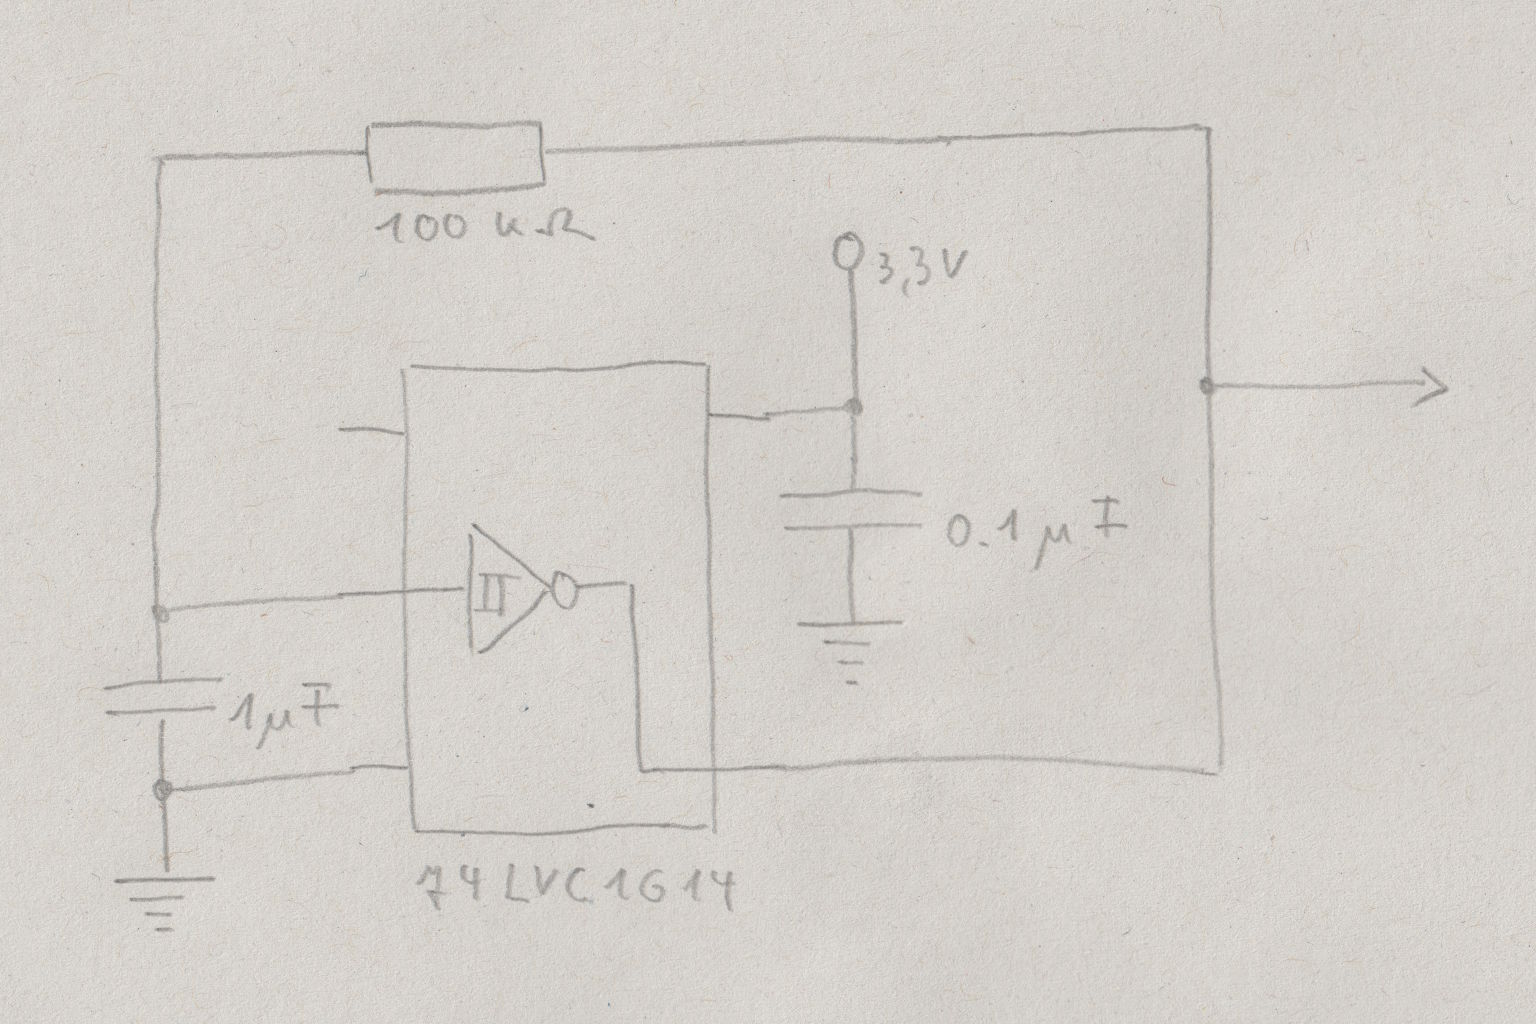
\includegraphics[scale=1.0]{auto-shutdown-timeout-hack.jpeg}}
	\caption{\label{auto-shutdown-timeout-hack}Oscillator for hack to disable auto-shutdown timeout}
\end{figure}

The oscillator can be built from just three small components: A 74LVC1G14 inverting Schmitt-trigger buffer, a 1 µF capacitor and a 100 k\si{\ohm} resistor (see Figure~\ref{auto-shutdown-timeout-hack}).

\end{document}

